\chapter{Externally Defined Variables}
\section{Moving Forward}
Let's create a new directory for this chapter, name it ''ChapterFour''. As the chapter implied, we now want to access variables that are defined in C Library, but unfortunately, C\# does not offer an easy approach to accomplish this, so we must look into Marshal static class that is provided in\newline ''System.Runtime.InteropServices'' namespace.

Let's create a new C source code file, ''ChapFour.c'' and open it with your favorite editor.

Add the following code to your source code:

\begin{lstlisting}{language=c}
#include <stdint.h>

int32_t MyVariable = 123;

void ResetMyVariable()
{
	MyVariable = 123;
}
\end{lstlisting}

You can compile the following code by running this command:

\begin{lstlisting}
clang -std=c99 -shared -fPIC -olibChapFour.so ChapFour.c
\end{lstlisting}
\newpage
You can export a list of symbols by running 
\begin{lstlisting}
objdump -T libChapFour.so
\end{lstlisting}

You will notice that we have a symbol for ''MyVariable''.

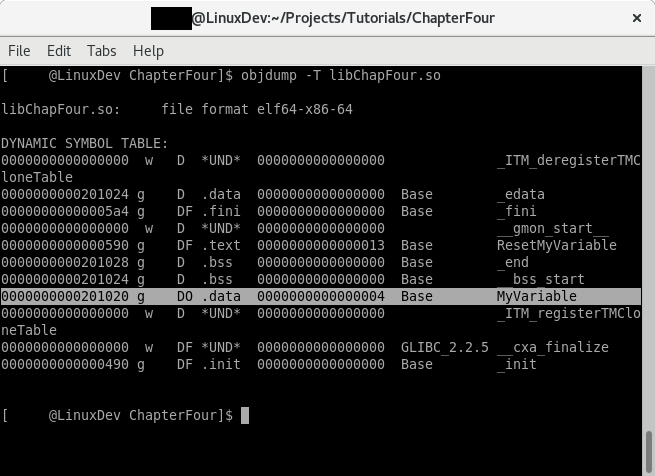
\includegraphics[width=\textwidth]{ChapFourConsole}

\section{Loading the Library Dynamically}
As mentioned above, we cannot normally access library that is loaded by the CLR already directly. In Mono Runtime, it will use DL library to load the library only once in this method, but \textbf{CoreCLR as of this time of writing (Nov 24, 2017) will load entirely new instance of library apart from DL library approach.}

Both DL library (for Linux Platform) and Kernel32.dll(Windows Platform) provide functions to load library and to return a handle for the same library if it is already previously loaded and haven't been freed first.

For the course of this chapter, we will load 3 new functions from DL library in order to enable us to access library that may already be loaded, dlopen, dlsym, and dlclose functions.

Let's get started by running the following command:

\begin{lstlisting}
dotnet new Console
\end{lstlisting}
\newpage
Open up ''ChapterFour.csproj'' file and add the following snippet under </PropertyGroup> tag inside <Project> tags.

\begin{lstlisting}{language=XML}
<Target Name="CompileCProject" AfterTargets="AfterBuild">
  <exec Command=
  "clang -std=c99 -shared -fPIC -olibChapFour.so
ChapFour.c" />
  <Copy SourceFiles="libChapFour.so" DestinationFolder="$(OutDir)" />
</Target>
\end{lstlisting}

Add the following line in <PropertyGroup> tags:

\begin{lstlisting}
<AllowUnsafeBlocks>true</AllowUnsafeBlocks>
\end{lstlisting}

Your ChapterFour.csproj should look like the following:

\begin{lstlisting}
<Project Sdk="Microsoft.NET.Sdk">

 <PropertyGroup>
  <OutputType>Exe</OutputType>
  <TargetFramework>netcoreapp2.0</TargetFramework>
  <AllowUnsafeBlocks>true</AllowUnsafeBlocks>
 </PropertyGroup>
 <Target Name="CompileCProject" AfterTargets="AfterBuild">
  <exec Command="clang -std=c99 -shared -fPIC -olibChapFour.so
ChapFour.c" />
  <Copy SourceFiles="libChapFour.so" DestinationFolder="$(OutDir)" />
 </Target>
</Project>
\end{lstlisting}
Now open ''Program.cs'' source code file and append the using directive at the top of the source code:

\begin{lstlisting}{language=c}
using System.Runtime.InteropServices;
\end{lstlisting}
\newpage
Now we need to load the externally defined functions for dynamically loading a library and to load the reset function from ''libChapThree.so'' library. Append the following codes inside Program class:

\begin{lstlisting}{language=c}
[DllImport("dl")]
static extern IntPtr dlopen(string file, int flag = 1);

[DllImport("dl")]
static extern IntPtr dlsym(IntPtr handle, string symbol);

[DllImport("dl")]
static extern int dlclose(IntPtr handle);

[DllImport("ChapFour")]
static extern void ResetMyVariable();

delegate void ResetMyVariable_dt();
\end{lstlisting}

Finally replace Main method with the following snippet:

\begin{lstlisting}
static unsafe void Main(string[] args)
{
	var libPath = "./libChapFour.so";
	IntPtr libraryHandle = dlopen(libPath);
	int* ptr = (int*)dlsym(libraryHandle, "MyVariable").ToPointer();
	Console.WriteLine("MyVariable Value: {0}", *ptr);
	
	*ptr = *ptr + 1;
	Console.WriteLine("Incremented Variable: {0}", *ptr);
	
	ResetMyVariable();
	Console.WriteLine("MyVariable after CLR Loaded ResetMyVariable Execution: {0}", *ptr);
	
	var resetVariable = Marshal.GetDelegateForFunctionPointer<ResetMyVariable_dt>
		(dlsym(libraryHandle, "ResetMyVariable"));
	resetVariable();
	Console.WriteLine("MyVariable after DL Loaded ResetMyVariable Execution: {0}", *ptr);
	
	dlclose(libraryHandle);
}

\end{lstlisting}
\newpage
There are few things happening here:

\begin{enumerate}
	\item ResetMyVariable\_dt is a delegate type declaration to convert a simple function pointer to a usable function in C\#. The \_dt suffix is acronym for delegate type.
	\item The optional parameter, flag, in dlopen function is default to RTLD\_LAZY flag which is 0x00001.
	\item Method must be marked as Unsafe whenever pointer datatype such as ''int*'' is used.
	\item Library Path is simply a path to the library that is in the current directory.
	\item The dlsym returns a pointer to the variable which then can be interacted with in C\# program and C library.
	\item When running this code in Mono and Dotnet Core, the result will be drastically different from one another. Mono will load the library only once and share the same handle while Dotnet core would create 2 different instances of the same library and therefore data that is defined in each library will not match.
\end{enumerate}

\newpage
Your source code for Program.cs should look like below:
\begin{lstlisting}{c}
using System;
using System.Runtime.InteropServices;

namespace ChapterFour
{
	class Program
	{
		[DllImport("dl")]
		static extern IntPtr dlopen(string file, int flag = 1);
		
		[DllImport("dl")]
		static extern IntPtr dlsym(IntPtr handle, string symbol);
		
		[DllImport("dl")]
		static extern int dlclose(IntPtr handle);
		
		[DllImport("ChapFour")]
		static extern void ResetMyVariable();
		
		delegate void ResetMyVariable_dt();
\end{lstlisting}
\newpage
\begin{lstlisting}{c}
		static unsafe void Main(string[] args)
		{
			var libPath = "./libChapFour.so";
			IntPtr libraryHandle = dlopen(libPath);
			int* ptr = (int*)dlsym(libraryHandle, "MyVariable").ToPointer();
			Console.WriteLine("MyVariable Value: {0}", *ptr);
			*ptr = *ptr + 1;
			Console.WriteLine("Incremented Variable: {0}", *ptr);
			ResetMyVariable();
			Console.WriteLine("MyVariable after CLR Loaded ResetMyVariable Execution: {0}", *ptr);
			var resetVariable = Marshal
				.GetDelegateForFunctionPointer
				<ResetMyVariable_dt>
				(dlsym(libraryHandle, "ResetMyVariable"));
			resetVariable();
			Console.WriteLine("MyVariable after DL Loaded ResetMyVariable Execution: {0}", *ptr);
			dlclose(libraryHandle);
		}
	}
}
\end{lstlisting}
\newpage
In dotnet core, we have the following:

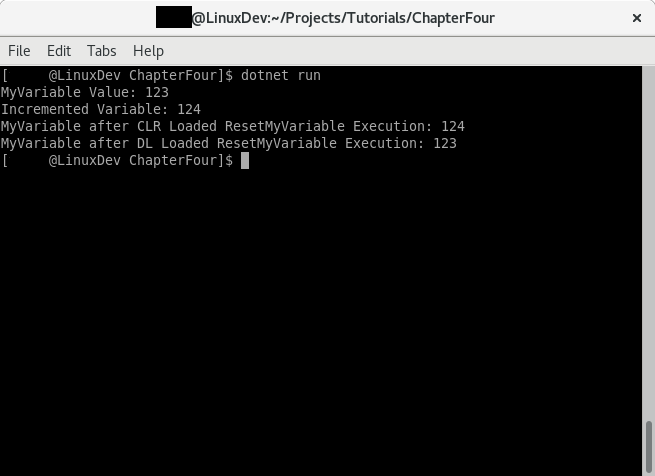
\includegraphics[width=\textwidth]{ChapFourConsoleOutputCore}

In Mono, we have the following:

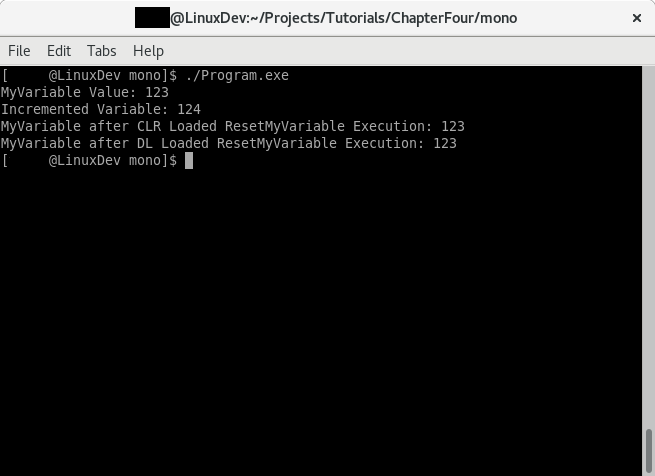
\includegraphics[width=\textwidth]{ChapFourConsoleOutputMono}
\newpage
\section{The Delegate Approach}
The difference is highlighted and as you can see, the result can be drastically different from one another and the behavior you see and expect in Dotnet Framework \textbf{WILL NOT} be consistent.
There is a different approach to tackle this particular issue.
We can limit our use of P/Invoke services provided by CLR to just loading DL library itself.
We can use DL library to load all externally defined functions and symbols within C\# and keep result and behavior consistent as demonstrated in both consoles above on the DL Loaded ResetMyVariable Execution line.
This approach is refered as the Delegate Approach.

\textbf{TODO}: Add Delegate Stub and Project to demonstrate how to work around the issue described above.